\begin{Exc}{(A5.16.v0, 5 points):}
Consider an alternative validity condition for binary consensus: There must
be at least one admissible execution with decision value 0, and there
must be at least one admissible execution with decision value 1.
Show that there is no wait-free algorithm for this modified consensus
problem in single-writer shared memory asynchronous systems.
\end{Exc}

% ------------------------------------------------------------------------------

\begin{Exc}{(L6.1.v0, 4 points):}
It is known that one can solve synchronous consensus
in the presence of $f=1$ Byzantine faulty processors
in a fully connected system of $n=4$ processors. Using an easy
impossibility proof, show that this is no longer possible when
two processors cannot communicate directly with each other.
\end{Exc}

\begin{proof}
Consider a graph $G$ (Figure \ref{fig:g}) with nodes $\{p_0, p_1, p_2, p_3\}$, in which
node $p_0$ has no direct connection to node $p_3$. Assume that an algorithm $A$
exists (s.t. node $p_i$ locally executes algorithm $A_i$ for all $i$)
that solves synchronous consensus with at most one Byzantine processor in system $G$.

\begin{figure}[ht]
\centering
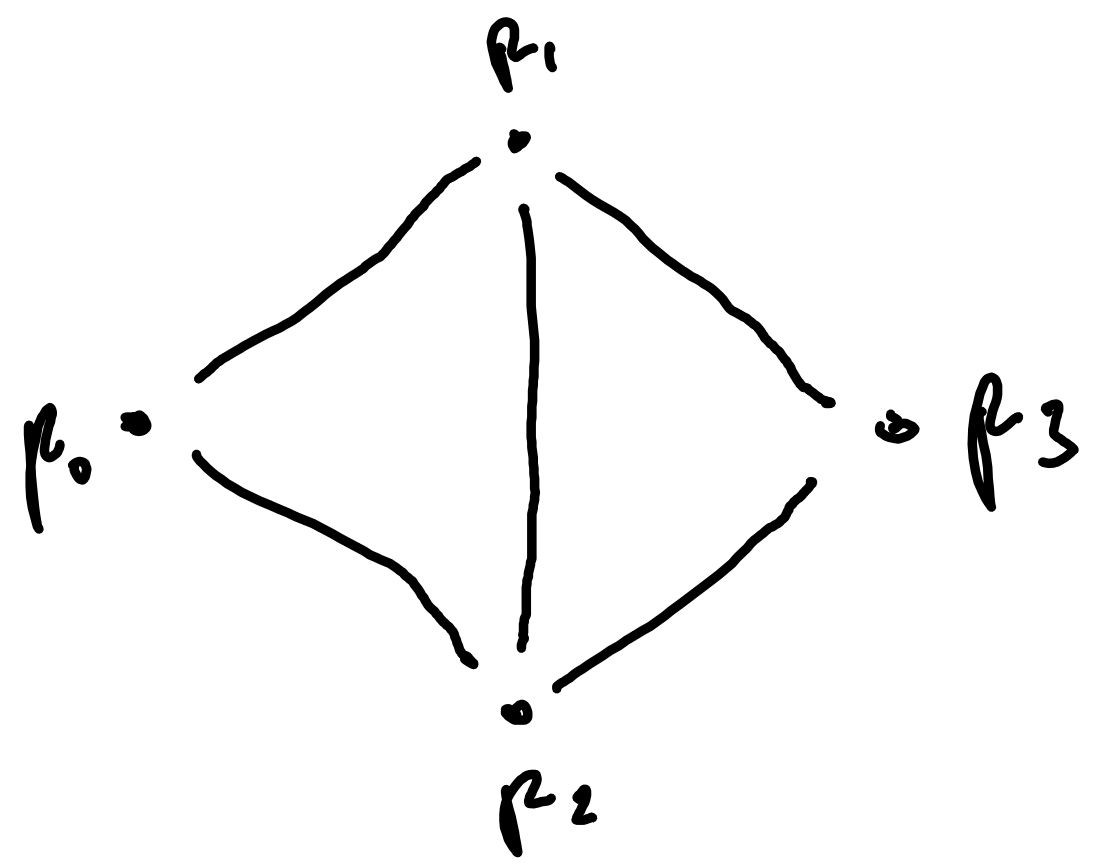
\includegraphics[width=0.5\textwidth]{fig_g}
\caption{The graph $G$. Nodes $p_0$ and $p_3$ are not connected.} \label{fig:g}
\end{figure}

Graph $G'$ (Figure \ref{fig:gprime}) is constructed in a way that is locally
indistinguishable from $G$ for each node. For all $i$, let nodes $p_i, p'_i$ execute $A_i$,
and let the input of nodes $\{p_0, p_1, p_2, p_3\}$ equal $0$ while the input of 
$\{p_0', p_1', p_2', p_3'\}$ equals $1$.

\begin{figure}[ht]
\centering
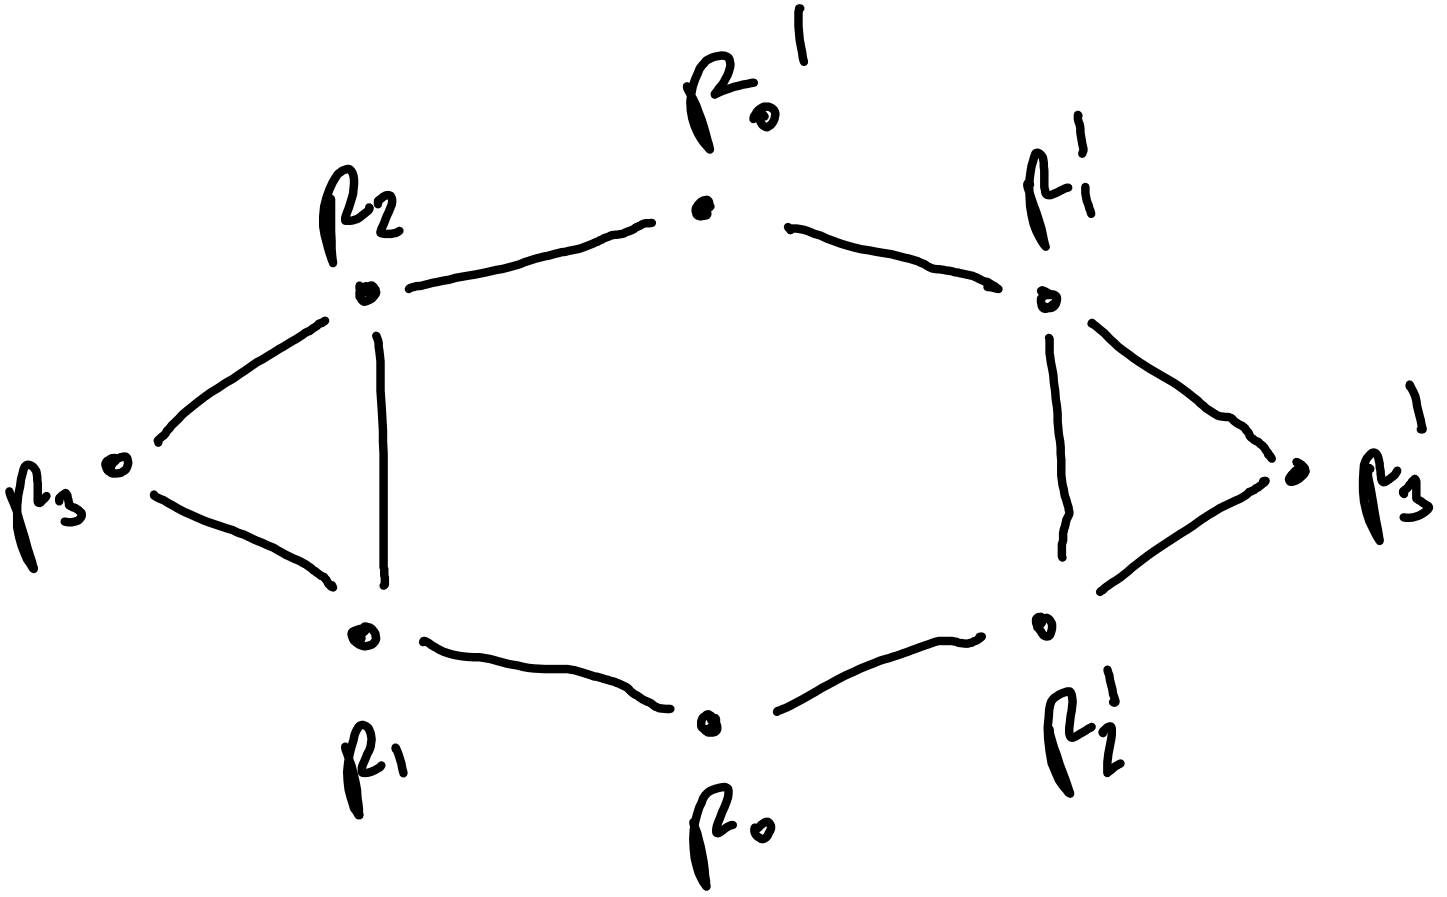
\includegraphics[width=0.5\textwidth]{fig_gprime}
\caption{The graph $G'$, locally indistinguishable from $G$.} \label{fig:gprime}
\end{figure}

Observe first the local subsystem $G'_0$ of $G'$ consisting of nodes $\{p_0, p_1, p_3\}$
plus the remaining edges to $\{p_2, p_2'\}$. This system equivalent to $G$ in which
node $p_2$ is faulty. By definition, $A$ can tolerate one Byzantine processor,
and by validity, all correct processors $\{p_0, p_1, p_3\}$ must decide $0$.

Similarly, the local subsystem $G'_1$ consisting of nodes $\{p_1', p_2', p_3'\}$
plus the remaining edges to $\{p_0, p_0'\}$ is equivalent to $G$ in which node
$p_0$ is faulty. Argumenting as above, nodes $\{p_1', p_2', p_3'\}$ must decide $1$.

Finally, observe the subsystem $G'_?$ consisting of nodes $\{p_0, p_2', p_3'\}$
plus the remaining edges to $\{p_1, p_1'\}$. Again, $G'_?$ is locally equivalent
to $G$ in which node $p_1$ is faulty. By agreement, all correct nodes must decide
$0$, or all correct processors must decide $1$.
However, we have previously established that processor $p_0$ decides $0$,
and processor $p_2$ decides $1$, a contradiction.

Therefore no such algorithm $A$ can exist.
\end{proof}

% ------------------------------------------------------------------------------

\begin{Exc}{(S.5.4.v0, 7 points):}
Consider a lockstep synchronous system, where processors never fail but
messages can be lost arbitrarily. Prove that it is impossible to solve
binary consensus with the alternative validity property
\begin{itemize}
\item If all processors start with the same
input value, then every processor~$p_i$ computes
\begin{itemize}
%\itemsep-2pt
\item $y_i=1$ if $\forall j: x_j=1$ and no message got
lost in the entire execution,
\item $y_i=0$ if $\forall j: x_j=0$,
\end{itemize}
\end{itemize}
in a system of $n=2$ processors. Does this impossibility also
hold for the following variants of consensus:
\begin{enumerate}
\item[(a)] Ordinary consensus, i.e., agreement, termination and
the standard validity property from the textbook?
\item[(b)] Consensus with unanimous termination, i.e., agreement and
validity from the textbook, and the requirement that
\begin{itemize}
\item if some processor decides, all processors eventually decide, plus
\item if no message is lost, all processors eventually decide?
\end{itemize}
\end{enumerate}
\end{Exc}

% ------------------------------------------------------------------------------

\begin{Exc}{(S.5.14.v0, 6 points):}
Consider synchronous consensus with at most $f$ crash failures in not
fully connected communication graphs $G$.
\begin{enumerate}
\item[(1)] Using a partitioning argument, prove that there is no solution for this problem if $G$
is not $f+1$-connected.
\item[(2)] Extend the proof of the termination time lower bound of $f+1$ rounds
for fully connected communication graphs: Prove that every algorithm ${\cal A}$
(that may know $G$) for $n\geq f+2$ processors needs at least $f+Radius(G)$ rounds
for termination.

Research problem (optional): You may win extra points by either improving this
bound (I conjecture that the actual bound is $f+Diam(G)$) or else
by giving an algorithm and a proof that it indeed terminates in
$f+Radius(G)$.
\end{enumerate}
\end{Exc}
